%\documentclass[preprint]{aastex}
\documentclass[twolcolumn,apj]{emulateapj}
\usepackage{ctable}
\usepackage{amsmath}
\usepackage{graphicx}
\usepackage{hyperref}
\usepackage{mathrsfs}
%\usepackage[figuresright]{rotating}
%\usepackage{rotating}
%\usepackage{natbib}
%\usepackage{pdflscape}
%\usepackage{lscape}
%\citestyle{aa}

\def\b{\mathbf{b}}
\def\k{\mathbf{k}}
\def\r{\mathbf{r}}
\def\q{\mathbf{q}}
\def\b{\mathbf{b}}
\def\kp{\mathbf{k}^\prime}
\def\kpp{\mathbf{k}^{\prime\prime}}
\def\V{\mathbb{V}}
\def\At{\tilde{A}}
\def\Vt{\tilde{V}}
\def\Tt{\tilde{T}}
\def\tb{\langle T_b\rangle}
\newcommand{\vis}{\mathbf{v}}
\newcommand{\x}{\mathbf{x}}
\newcommand{\xhat}{\hat{\mathbf{x}}}
\newcommand{\A}{\mathbf{A}}
\newcommand{\y}{\mathbf{y}}
\newcommand{\N}{\mathbf{N}}
\newcommand{\Nfg}{\mathbf{N}_{\textrm{fg}}}
\newcommand{\Q}{\mathbf{Q}}
\newcommand{\M}{\mathbf{M}}
\newcommand{\W}{\mathbf{W}}
\newcommand{\G}{\mathbf{G}}
\newcommand{\R}{\mathbf{R}}
\newcommand{\F}{\mathbf{F}}
\newcommand{\rhat}{\hat{\mathbf{r}}}
\newcommand{\Nbl}{N_{\textrm{bl}}}

\newcommand{\acl}[1]{{\color{red} \textbf{[ACL:  #1]}}}
\definecolor{applegreen}{rgb}{0.55, 0.71, 0.0}
\newcommand{\mep}[1]{{\color{applegreen} \textbf{[MEP:  #1]}}}

\renewcommand{\topfraction}{0.85}
\renewcommand{\bottomfraction}{0.1}

\begin{document}

%\title{What Power Spectrum Measurements From the Next Generation of 21~cm Experiments Can Teach Us About the Epoch of Reionization}
\title{Global signal interferometer (XXX: replace with better title)}

\author{Morgan E. Presley\altaffilmark{1},
}
\altaffiltext{1}{Department of Astrophysical Sciences, Princeton University, Princeton NJ}

\begin{abstract}
Really great abstract
\acl{Hey, look at these fun commands.}
\mep{Here's yours.}
\mep {Check out all the colors!!! http://latexcolor.com/}
\end{abstract}


\keywords{reionization, dark ages, first stars --- techniques: interferometric}

\section{Introduction}
\acl{DID WE REMEMBER TO DIVIDE THE $a_{00}$ values by $\sqrt{4\pi}$?}
\begin{itemize}
\item Say why 21cm is important.
\item Narrow focus to global signal.  Show a plot of the signal.
\end{itemize}

\begin{figure}[h]
	\centering
	%\includegraphics[width=0.55\textwidth]{}
	\caption{\mep{Insert 21cm signal evolution figure.}}
	\label{fig:21cmSignal}
\end{figure}

Figure \ref{fig:21cmSignal} shows a schematic of a fiducial model of the global 21 cm signal, highlighting the important epochs and corresponding features in the signal. The first epoch, the cosmic ``Dark Ages,'' arises with the thermal decoupling of the 21 cm spin states from the cosmic microwave background (CMB) and is marked by a shallow absorption feature. As the gas density continues to fall with the universe's expansion, collisions are no longer able to couple the spin states to the gas, and the signal falls back into coupling with the CMB. The next epoch is marked by the formation of the first stars and galaxies, whose Ly$\alpha$ photons strongly couple the spin states to the gas temperature. This first results in a deep absorption feature, as the gas temperature is far below that of the CMB. However, heating from X-ray emission pushes the gas above the CMB temperature, resulting in a 21 cm emission signal. This leads to the final epoch, the ``epoch of reionization,'' where UV photons ionize the gas, gradually erasing the 21 cm signal. \mep{Do I need to cite \citet{Pritchard_Loeb_21cm_Review} since I used them for reference when writing this?} 

\begin{itemize}
\item Challenge of foregrounds.  \acl{We should probably also comment on the ionosphere at some point}.
\item Survey of current instruments and efforts. (EDGES, DARE, SCI-HI, LOFAR, LEDA, LWA) \acl{Gotta also survey some of the other experiments that one doesn't hear about so much.  Gianni's paper has a good list.  Also be sure to add more references like Jack Burns' ScienceDirect article.}
\end{itemize}
There are currently a large number of experiments seeking to make a first detection and characterization of the global $21\,\textrm{cm}$ signal.  The Experiment to Detect the Global EoR Signal (EDGES) uses an extremely well-calibrated single dipole \citep{rogersCalib} to integrate over large parts of the sky, producing a global spectrum from $100$ to $200\,\textrm{MHz}$.  Modeling foreground spectra as a sum of low-order polynomials, EDGES has placed a lower limit of $\Delta z > 0.06$ on the duration of reionization \citep{bowmanRogersMeasurement}.  Similar in concept but operating at a lower frequency range of $55$ to $99\,\textrm{MHz}$ is the Sonda Cosmol\'{o}gica de las Islas para la Detecci\'{o}n de Hidr\'{o}geno Neutro (SCI-HI) experiment.  This frequency range corresponds to the redshift range $13.3 < z < 24.9$, providing access to the prominent dip in the signal prior to reionization.  Using a similar polynomial foreground subtraction technique to EDGES, SCI-HI is able to achieve a foreground residual level of $\sim 10\,\textrm{K}$ at $\sim 70 \,\textrm{MHz}$ \citep{voytekSCIHI}.

To escape radio frequency interference (RFI), both EDGES and SCI-HI are deployed in rather remote locations: EDGES observes from the Murchison Radio-astronomy Observatory in Western Australia, while SCI-HI has been deployed at Isla Guadalupe in Mexico, with plans to observe at Isla Socorro and/or Isla Clari\'{o}n in the future.  To achieve even better RFI isolation (as well as to escape ionospheric distortions), the Dark Ages Radio Explorer (DARE) satellite has been proposed \citep{DAREMCMC}.  DARE consists of a short dipole antenna in lunar orbit, which allows the Moon to be used an RFI shield.  DARE probes a frequency range of $40$ to $120\,\textrm{MHz}$, again providing direct access to the pre-reionization epoch.

Moving beyond single dipole experiments, the Large-aperture Experiment to detect the Dark Ages (LEDA) makes use of an interferometric array of antennas to simultaneously model the sky and calibration parameters \citep{BernardiLEDA}.  Fundamentally, however, its measurement of the global signal is still expected to come from total power measurements (i.e., auto-correlations) from single dipoles treated independently.  This differs from the approach taken by \citet{VedanthamLOFAR2}, where the LOw Frequency ARray (LOFAR) was operated as a true interferometer not just for calibration purposes, but also for the cosmological measurement itself.  At a basic level, one might imagine that interferometers are sensitive only to spatially fluctuating signals on the sky (if one follows the standard procedure of avoiding noise bias by discarding auto-correlations in the data), and are therefore insensitive to the global signal.  However, an externally imposed spatial dependence can introduce sufficient spatial structure for a global signal to be measurable by an interferometer.  \citet{VedanthamLOFAR2} took advantage of this fact by observing fields containing the Moon, effectively using lunar occultations to introduce the necessary spatial dependence for an interferometric measurement of the global signal.  So far, this approach has yielded a reasonably high signal-to-noise characterization of the foreground contaminants between $\nu =35$ and $80\,\textrm{MHz}$.

\begin{itemize}
\item Why an interferometer might be helpful plus why we're not crazy (Ekers + Rots Theorem?).  Angular info helps with foreground suppression.
\end{itemize}
\acl{Somewhere, need to address the point that time integration can allow extra information to be gleaned.}

In this paper, we build on \citet{VedanthamLOFAR2}, generalizing their work to consider a general theory of interferometric measurements of the global $21\,\textrm{cm}$ signal.  We provide a mathematically rigorous framework for extracting the global signal from an interferometer.  Given that interferometers naturally sample spatial information, a global signal measurement that is made by an interferometer is well-poised to use angular information to separate foregrounds from the (monopole) cosmological signal.  As pointed out in \citep{L13} and \citep{Liu_Switzer_2014}, the angular dependence of foregrounds can be leveraged to enable better foreground subtraction.  In this present paper we use our mathematical formalism to show how such a scheme may be implemented in the specific context of an interferometric measurement.  Although we find that some amount of spectral foreground subtraction is still necessary, our Monte Carlo simulations show that spatial information can reduce the burden of the spectral subtraction, reducing the risk of cosmological signal loss.  \acl{Should probably have brought up cosmological signal loss and angular subtraction earlier}  Fisher matrix projections confirm the stringent constraints on the Dark Ages and reionization that can be obtained with our approach.  \acl{Probably want a statement stronger than this.}

\begin{itemize}
\item Preview results (exquisite extraction; great foreground mitigation; high significance detection).
\end{itemize}

The rest of this paper is organized as follows.  In Section \ref{sec:QualitativePic} we provide some qualitative intuition for using interferometry to measure monopole signals.  This is made more mathematically rigorous in Section \ref{sec:MathForm}, where we establish a matrix-based framework for signal extraction.  Section \ref{sec:Foregrounds} introduces foregrounds and our strategy for their mitigation.  Its effectiveness is demonstrated using Monte Carlo simulations in Section \ref{sec:MonteCarlos}.  The Monte Carlo results are then propagated through to theory parameters in Section \ref{sec:Fisher} using a Fisher matrix formalism.  We summarize our conclusions in Section \ref{sec:Conc}.

\section{Why we're really not crazy}
\label{sec:QualitativePic}
\begin{itemize}
\item Cartoon / qualitative picture? \mep{Remind me -- What was this pic supposed to show?}
\item Simple eqn. showing that there is non-zero response?
\item Intuitive, qualitative description of what sort of arrays are good.  (Preview for later sections).
\item Discussion of noise bias and other problems with single dipole experiments?
\end{itemize}

\section{Mathematical formalism}
\label{sec:MathForm}
\begin{itemize}
\item How does one actually get from visibilities to a global signal measurement.
\item The error statistics that come for free.
\item Quantification of leakage from other spherical harmonics.
\end{itemize}

%\acl{I'd like to say a little earlier that we're trying to get the first component of $\mathbf{x}$.  I'd also like to state in this section that we're envisioning doing this frequency-by-frequency first.  In other words, Equation 1 applies at a particular frequency.  It didn't have to be like this.  We could've expanded the dimensions of equation 1 to include all frequencies in a gigantic linear system of equations.  We're doing things freq-by-freq in order to be very conservative, since we don't want to make too many assumptions about the spectrum when the thing we're trying to measure is a spectrum.}
In order to obtain a global signal measurement from visibilities, it is necessary to invert the linear equation 
\begin{equation}
\y = \Q \mathbf{x} + \mathbf{n}
\label{eqn:yQxn}
\end{equation}
where $\y$ is a vector of length $\Nbl$ containing the visibilities measured at different baselines, $\mathbf{n}$ is the contribution of noise from both foregrounds and systematics, and $\mathbf{x}$ is a projection of the true sky onto the spherical harmonics $Y_{\ell m}(\theta,\phi)$. As such, $\mathbf{x}$ has length $(\ell_{\textrm{max}}+1)^2$, where $\ell_{\textrm{max}}$ is the largest $\ell$ value used in the model of the true sky. The global signal corresponds only to the first component of $\mathbf{x}$, where $\ell,m=0,0$. However, since the sky is composed of the overlay of many higher-order structures, it is \mep{advisable? necessary?} to also fit higher $\ell$'s and $m$'s. 

The matrix $\Q$ is the beam response of an antenna array at different baselines (rows) and different spherical harmonics (columns). $\Q$ is determined by 
\begin{equation}
\textrm{Q}_{j,\ell m} = \int d\Omega A(\boldsymbol \theta) Y_{\ell m}(\boldsymbol \theta) e^{-2\pi i \frac{\mathbf{b_\textit{j}}}{\lambda} \cdot \boldsymbol \theta}
\label{eqn:Qdef}
\end{equation}
where $\boldsymbol \theta$ is the angular position on the sky, $A$ is the primary beam for the antennas, $\mathbf{b_{\textit{j}}}$ is the $j$th baseline, and $\lambda$ is the wavelength of observation. Note that in the formulation of Eqs. \eqref{eqn:yQxn} and \eqref{eqn:Qdef} we assumed that all calculations would be done at a specific frequency. This is not necessary, as we could have expanded the dimensions of Eq. \eqref{eqn:yQxn} to include all of the frequencies measured in the experiment. However, we chose to do our calculations for each frequency independently in order to remain conservative in our assumptions about the spectrum.

Since $\Q$ is not in general invertible, we cannot solve Eq. \eqref{eqn:yQxn} for $\mathbf{x}$ directly and instead can only recover an estimator for $\mathbf{x}$. We can define a general estimator of the form 
\begin{equation}
\mathbf{\hat x} = \M \Q^\dagger \N^{-1} \y
\label{eqn:xhat}
\end{equation}
where $\N$ is the total noise covariance matrix and M is some matrix chosen by the data analyst. One useful choice for $\M$ is 
\begin{equation}
\M = [\Q^\dagger \N^{-1} \Q]^{-1}
\label{eqn:M}
\end{equation}
which is obtained through a least-squares derivation that minimizes $\chi^2 \equiv (\y-\Q \mathbf{\hat x})^\dagger \N^{-1} (\y-\Q \mathbf{\hat x})$. Note that for this choice of $\M$, the ensemble average of $\mathbf{\hat x}$ is $\mathbf{x}$.
Using this fact, we can directly find the covariance of $\mathbf{\hat x}$ to be 
\begin{equation}
\textrm{Cov}(\mathbf{\hat x}) = [\Q^\dagger \N^{-1} \Q]^{-1}
\label{eqn:Covxhat}
\end{equation}
as shown in \citet{Tegmark_CMB_maps_wli}. Therefore, using equation (\ref{eqn:M}) for our statistical analysis allows us to analytically find the error statistics if the noise covariance matrix for the foregrounds and systematics is known. However, since galactic foreground models are not well constrained, it is not safe to assume we know $\N_{\textrm{fg}}$. Consequently, Monte Carlo simulations are still necessary to determine the error bars on measurements analyzed using this method. Note, however, that although we do not know the exact noise covariance $\N$, there is nothing wrong with choosing Eq. \eqref{eqn:M} for our data analysis, as long as we do not claim that our error bars are constrained by equation (\ref{eqn:Covxhat}). %-- it just may not be optimal.

Note that two inverses must be taken in order to compute $\M$. In general, $\Q^\dagger \N^{-1} \Q$ will not be invertible, requiring us to approximate the inverse with a pseudo-inverse. We used a pseudo-inverse method that raises the value of the small eigenmodes, inverts, and then projects out those small eigenmodes, as laid out in the appendix of \citet{Tegmark_CMB_spectra_wli}. 

Since $\Q$ is not diagonal, higher spherical harmonic modes will leak into our measurement $\y$. If it were possible to do the inverses in equation \ref{eqn:M}, then these leakages could be dampened down by taking repeated observations to mimic an ensemble average. This is because 
\begin{equation}
\langle \xhat \rangle = \M \Q^\dagger \N^{-1} \Q \x
\end{equation}
which is equal to $\x$ if $\M$ is the true inverse of $\Q^\dagger \N^{-1} \Q$. In order to quantify the relative amount of leakage from the different modes, it is convenient to define a window function matrix $\W$ as 
\begin{equation}
\W = \M \Q^\dagger \N^{-1} \Q. 
\end{equation}
With this definition, the elements of the first row of the window function matrix quantifies the ratios between the contributions from the different modes. A good experimental design would result in a very high ratio between $W_{0,00}$ and all of the other $W_{0,\ell m}$.

\mep{Figure time! Show the green/pink plots of 1st row of window function for different arrays.}
\acl{I'm wondering if it might actually be good to display the window function plots in a way that's averaged over $m$, since for a given $\ell$ the $m$ value basically just changes the direction.  One could imagine something analogous to the angular power spectrum, which is often estimated by computing $\hat{C}_\ell = \frac{1}{2\ell + 1} \sum_{m=-\ell}^{\ell} |a_{\ell m}|^2$.  We could do an analogous sum.  On the other hand, the baseline vector breaks the symmetry and does pick out a direction.  So if we want to build that intuition, it could be useful to show the different $m$ values separately.}

\begin{figure}[h]
	\centering
	\includegraphics[width=0.55\textwidth]{figures/W_matrix_filler.pdf}
	\caption{\mep{Of course, this will have to be updated when the new data comes in. Probably to show several figures for different arrays?}\mep{Uh.... Weird stuff happens if I try to make the figure bigger. It's not wrapping the text and is trying to keep the figure in the column somehow?? Not sure what's up with the formatting style here.}\acl{Is this better? Or did you actually want to make this a figure that spans both columns? If so, change ``figure" to ``figure*" when you do \textbackslash begin.}}
	\label{fig:WindowFunction}
\end{figure}

\acl{The tone of the writing is excellent, btw.}
%
%\section{Exploration of arrays}
%\begin{itemize}
%\item Show plots of different arrays that we tried.
%\item (Maybe spherical harmonic plots with fringe patterns overlaid on spherical harmonics).
%\item Reasoning behind our crazier-looking arrays.
%\item Rules of thumb for designing a global signal interferometer.
%\end{itemize}

\section{Foregrounds and their mitigation}
\label{sec:Foregrounds}
\begin{itemize}
\item General characteristics of foregrounds.
\item Desire to avoid using too much spectral information because the signal itself is a spectrum.
\item How to use angular information.
\item (Modifications to array design to account for foregrounds).
\end{itemize}

The primary source of contamination in a global signal experiment comes from galactic foregrounds, which make extraction of the global signal difficult for a number of reasons. Primarily, the galactic foregrounds are many orders of magnitude brighter than our expected signal, so finding the global signal through a simple spatial average over the sky would result in a measurement dominated by foregrounds. Also, since both the galactic foregrounds and the expected global re-ionization signal are spectrally smooth, foreground subtraction techniques will likely be unreliable. Therefore, we propose using angular information to differentiate galactic foregrounds from the global signal. 

In order to best remove the foregrounds from our data, we construct a noise covariance matrix for the foregrounds: $\Nfg$. $\Nfg$  shows the correlation between the Fourier modes probed by the antenna array, and hence has dimensions $\Nbl \times \Nbl$. One method \mep{Are there other methods?} to generate $\Nfg$ from a model of the sky is to first find a covariance matrix of the sky $\R$ and transform that matrix into the Fourier domain of the visibilities via the matrix transformation 

\begin{equation}
\Nfg = \mathbf{G} \R \mathbf{G}^\dagger
\label{eqn:Nfg}
\end{equation}
Since $\R$ has dimensions $N_{\textrm{pix}} \times N_{\textrm{pix}}$, note that $\mathbf{G}$ must have dimensions $\Nbl \times N_{\textrm{pix}}$. Although $\mathbf{G}$ serves a purpose similar to a Fourier transformation matrix, it is not precisely a Fourier matrix as that would probe every single possible Fourier mode, and we only want those that correspond to our array's baselines. As such, $\mathbf{G}$ is defined by 
\begin{equation}
G_{i,j} = A(\rhat_j)e^{-2\pi i \frac{\mathbf{b_\textit{i}}}{\lambda} \cdot \boldsymbol \rhat_j} \Delta \Omega
\end{equation}
where $\rhat_j$ is the angular position of the $j$th pixel,  $\Delta \Omega$ is the solid angle encompassed by each pixel, and $\mathbf{b_\textit{i}}$ is the $i$th baseline. 

\mep{Insert here stuff on how you're calculating $\R$?}

Once $\mathbf{G}$ has been found, all that remains is to find the covariance in the image space: $\R$. A naive model for the image covariance would be to create a diagonal matrix defined by 
\begin{equation}
\R_{i,i} = m^2(\rhat_i)
\end{equation}
where $m^2(\rhat_i)$ is the brightness of the sky \mep{Is this true?} at the pixel with angular position $\rhat_i$. This model can be useful because it ensures that there will be non-diagonal correlations in the spherical harmonic space and because it makes equation (\ref{eqn:Nfg}) easy to compute. However, a diagonal covariance is not a realistic portrayal of the true sky, since each pixel is clearly correlated to the ones near it. 

At the other extreme, 

\acl{An interesting point I just realized.  We can make the argument that since the normalization of $\mathbf{N}$ scales out of the expression for $\hat{\mathbf{x}}$, our foreground mitigation scheme is a very conservative one that only uses shape information, and not the detailed spectral form of our foreground model.}
\acl{Somewhere, we also need to address rotation synthesis}
\acl{Also need to add noise to simulations}.

\section{Monte carlo / foreground simulation results}
\label{sec:MonteCarlos}

\acl{TODO: Let's be conservative and try to do some arrays that are quite widely spaced and also to add some curvature into our Monte Carlos.  Plus frequency-dependent beams.}
\acl{TODO: Do some pictures of spherical harmonics in the Mollweide projection to build some intuition.}

\begin{itemize}
\item $\mathbf{N}_\textrm{fg}$ might not be properly modeled, so we can't use $[\mathbf{Q}^\dagger \mathbf{N}^{-1} \mathbf{Q}]^{-1}$ as a reliable indicator of the errors.  (Although recall that it's a perfectly fine choice for extracting the signal).
\item To get reliable estimates...Monte Carlo!
\item Really great results! (Error bars and covariance on the recovered spectra).
\end{itemize}

Recall from Section \ref{sec:MathForm} that using the least-squares method for recovering $\xhat$ allows us to analytically determine the error covariance of $\xhat$ via Eq. \eqref{eqn:Covxhat}. However, this formula for the covariance is only true if we exactly know the noise covariance matrix. Thus, since $\Nfg$ might not be properly modeled, we must still resort to Monte Carlo simulations to determine the error bars on our measurements. 

Our Monte Carlo simulations generate many visibilities $V(\mathbf{b}_i)$ from randomly perturbed sky models. \mep{Is ``randomly perturbed'' an appropriate way to describe it?} The sky models are derived by taking the all-sky survey from \citet{Haslam_408MHz_map} and using the power-law model of the foreground spectrum used in \citet{Liu_21cm_Fg} to extrapolate a map at the desired frequency. For a pixel at $\boldsymbol \theta$, the brightness at a certain frequency $\nu$ is 
\begin{equation}
I(\boldsymbol \theta) = I_H(\boldsymbol \theta) \left ( \frac{\nu}{\nu_H} \right ) ^{-\alpha + \Delta \alpha}
\end{equation}
where $I_H$ is the sky map from \citet{Haslam_408MHz_map}, $\nu_H=408$MHz, $\alpha = 2.8$, and $\Delta \alpha$ is a perturbing index randomly generated with variance 0.1. From this model, we can generate a vector of visibilities for all of the different baselines in an array. This vector is $\y$ from Eq. \eqref{eqn:yQxn}. The visibilities are defined as 
\begin{equation}
V(\mathbf{b}_i) = \int d \Omega A(\boldsymbol \theta) I(\boldsymbol \theta) e^{-2\pi i\frac{\nu}{c} \mathbf{b}_i \cdot \boldsymbol \theta}
\end{equation}
where $\boldsymbol \theta$ is the angular position on the sky, $A$ is the primary beam for the antennas, $\mathbf{b_{\textit{j}}}$ is the $j$th baseline, $\nu$ is the frequency of observation, and $I$ is the intensity \mep{What's the correct name for this?} of the sky model. 

Once we have generated a $\y$ vector, we can use Eq. \eqref{eqn:xhat} to find the estimator for the global signal that our analysis would produce for that particular sky. The variance of a large set of estimators from many such sky models provides us with the error bars for an experiment measuring the global signal. \mep{I don't like the phrasing of this paragraph.} 

\section{Fisher matrix results}
\label{sec:Fisher}
\begin{itemize}
\item Fisher matrix formalism for translating error statistics from recovered spectra to parameterizations of the signal.
\end{itemize}

While the Monte Carlo simulations give us constraints on how well a certain experiment (defined by a given $\Q$ and $\N$) can measure the global signal $\hat \x_{00}$, they do not provide us with constraints on scientifically relevant cosmic parameters. In order to find how well an experiment could constrain parameters relevant to the time evolution of the global signal, we employ a Fisher matrix formalism. The Fisher information matrix is defined as 
\begin{equation}
\F_{i,j} = \left \langle \frac{\partial \mathscr{L}(\boldsymbol \theta | \x)}{\partial \theta_i \partial \theta_j} \right \rangle
\end{equation}
where $\mathscr{L}(\boldsymbol \theta | \x)$ is the likelihood of a set of parameters $\boldsymbol \theta$ given the measurements $\x$ \acl{Careful: the thing that you differentiate to get the Fisher matrix is the *log* likelihood}. Given a Gaussian likelihood function with covariance matrix $C$ and centered on a model $\boldsymbol \mu(\boldsymbol \theta)$, and assuming that the measurements are unbiased, the elements of the Fisher matrix become
\begin{equation}
\F_{i,j} = \frac{\partial \boldsymbol \mu ^t}{\partial \theta_i} C^{-1} \frac{\partial \boldsymbol \mu}{\partial \theta_j}
\end{equation}
Note that the inverse of the Fisher matrix is the covariance of the parameters. Therefore, the error in $\theta_i$ is on the order of $\sigma_i \sim \sqrt{(\F^{-1})_{ii}}$. 

Now, this methodology has assumed that the measurements are unbiased, i.e. $\langle \xhat \rangle = \boldsymbol \mu (\boldsymbol \theta)$. If the measurements are biased by $\delta \xhat$, then the parameters will be biased by 
\begin{equation}
\delta \theta_i = \sum_{j} (\F^{-1})_{ij} \frac{\partial \boldsymbol \mu ^t}{\partial \theta_j} C^{-1} \delta \xhat 
\end{equation}
Note that the dimensions here work out because $\delta \xhat$ and $\boldsymbol \mu(\boldsymbol \theta)$ have length $N_\textrm{fq}$, and $C^{-1}$ has dimensions $N_\textrm{fq} \times N_\textrm{fq}$.  

Using the Fisher matrix formalism, we analyzed how well different arrays would be able to constrain models for different epochs in the evolution of the global signal. %\mep{It seems at this point that it would be helpful to refer to a picture of the fiducial model of the global signal, such as the one in your designer's guide paper. Actually, should we in an earlier section describe in more detail what we think the signal will look like? If so, where would that be? In the introduction?} \acl{Yep, I think the intro is the right place for it.  Earlier today I sneakily added a second sentence to the second bullet point there.} 
At about $z\sim 30$ when the first galaxies form, we expect a significant absorption feature as Lyman-alpha photons couple the spin and gas temperatures (see Fig. \ref{fig:21cmSignal}). This dip can be modeled as a Gaussian in frequency
\begin{equation}
\boldsymbol \mu = -A\textrm{exp}\left ( -\frac{(\nu - \nu_0)^2}{2\sigma^2} \right ) 
\end{equation}
so that the parameter vector is $\boldsymbol \theta = (A,\nu_0,\sigma)$, where $A$ is the amplitude of the signal, $\nu_0$ is the center of the absorption dip, and $\sigma$ is the width. Given a model and a fisher matrix, we can approximate the likelihood function of the parameter values as a multivariate Gaussian with covariance $\F^{-1}$.  
\begin{equation}
L(\boldsymbol \theta) \approx \frac{1}{(2\pi)^{n/2}(\textrm{det} \F^{-1})^{1/2}} \textrm{exp} \left ( -\frac{1}{2}(\boldsymbol \theta - \boldsymbol \theta_{\textrm{m}})^t \F (\boldsymbol \theta - \boldsymbol \theta_{\textrm{m}}) \right )
\end{equation}
where $n$ is the length of the parameter vector and $\boldsymbol \theta_{\textrm{m}}$ are the parameters with maximum likelihood. In order to more easily visualize the 3-dimensional contours of $L(\boldsymbol \theta)$, we examine the parameters pairwise by integrating over the third parameter in order to produce a new 2-dimensional likelihood function. Fig. \ref{fig:contours} shows contours of such pairwise likelihood functions for ... 

\mep{Insert figures of pairwise projections and discussion thereof.} 

\begin{figure}[h]
	\centering
	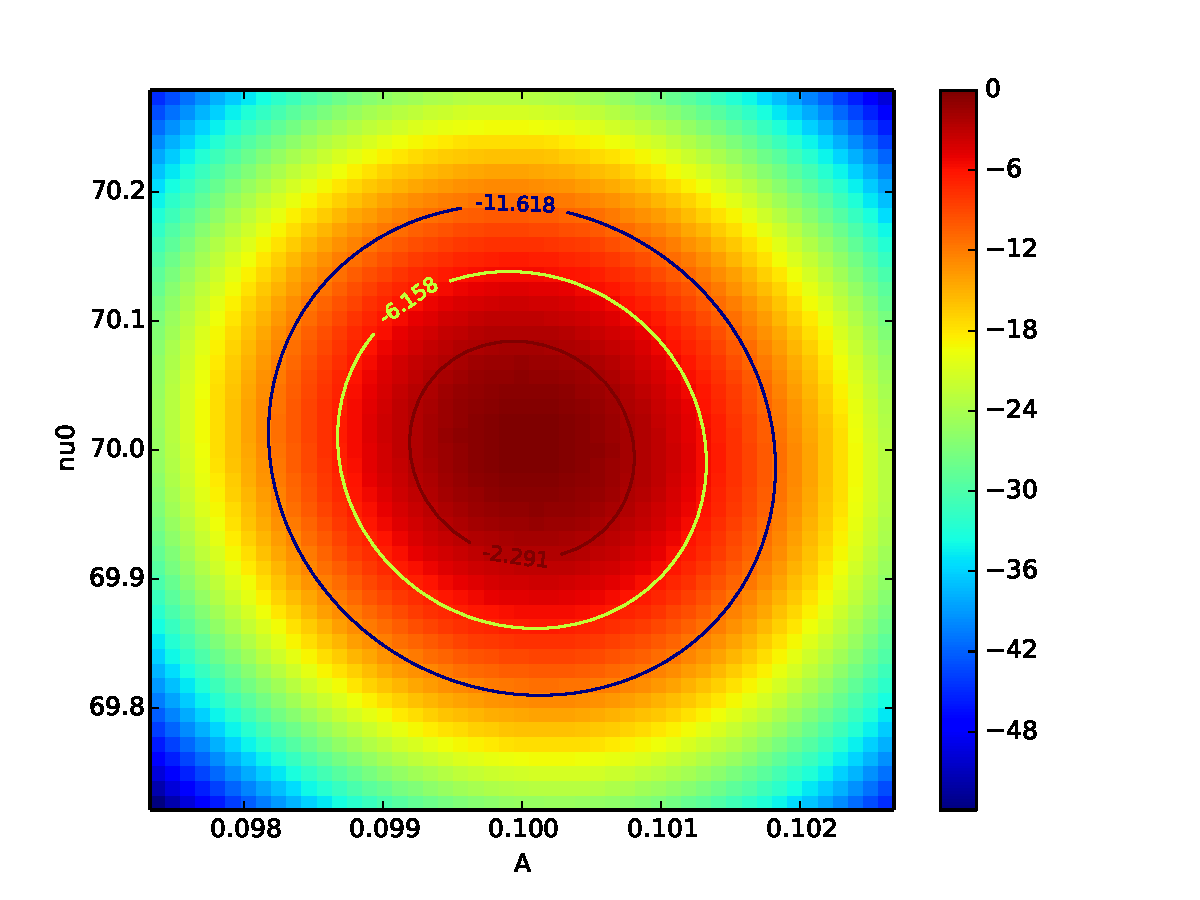
\includegraphics[width=0.55\textwidth]{figures/contours_A_nu0.pdf}
	\caption{\acl{Fill this in.  Probably also want to make this a horizontal stripe of constraints.}}
	\label{fig:contours}
\end{figure}

\begin{figure}[h]
	\centering
	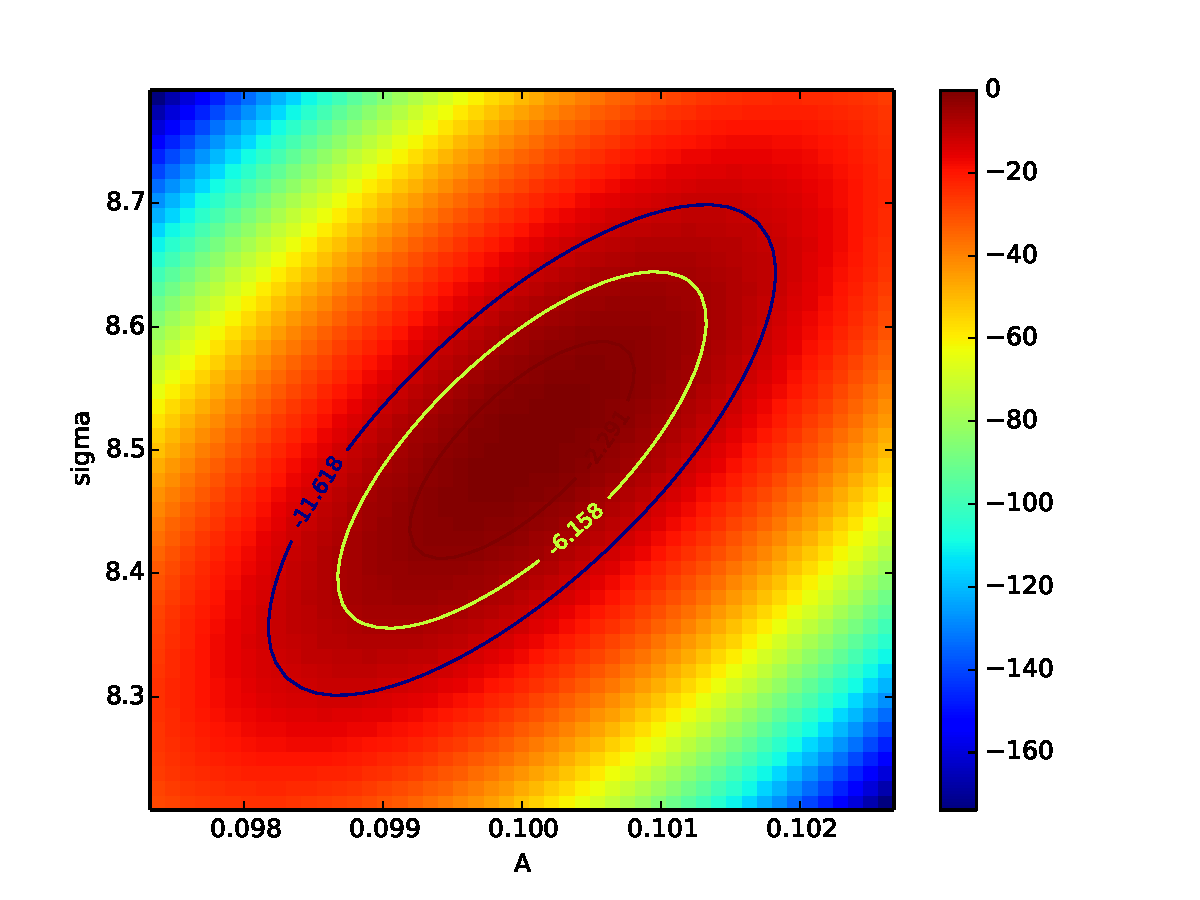
\includegraphics[width=0.55\textwidth]{figures/contours_A_sigma.pdf}
	\caption{\acl{Fill this in}}
\end{figure}

\begin{figure}[h]
	\centering
	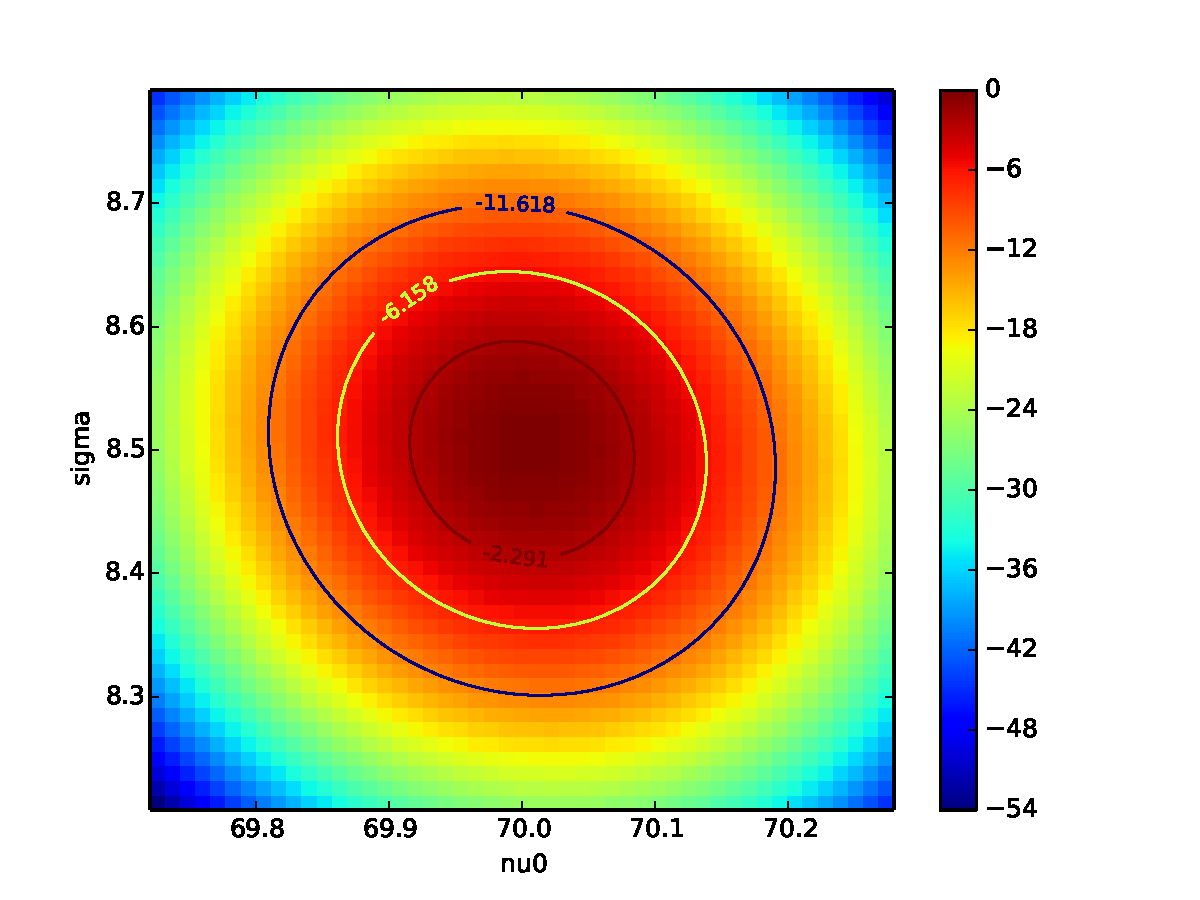
\includegraphics[width=0.55\textwidth]{figures/contours_nu0_sigma.pdf}
	\caption{\acl{Fill this in}}
\end{figure}

\section{Conclusions}
\label{sec:Conc}
\acl{On the theme of better relating this to a broad audience, we can also relate this to the high redshift galaxy people.  If their (collective) constraints are to be believed, there should be a sharp rise in ionization fraction at a redshift that's *just* below what EDGES is able to constrain.  So perhaps this can be motivation for building a global signal experiment that can confirm/refute the optical and IR people}
\begin{itemize}
\item This is a great way to do this measurement.  It will produce lots of great science! And eternal glory!
\end{itemize}

\bibliographystyle{apj}
\bibliography{globalSig}{}

\end{document}
